\chapter{引言}
\section{研究背景和意义}
地震勘探的主要目标是通过观测到地震数据来定量地估计地下模型实现对储层分布的准确预测。
弹性参数,包括纵波(P波)速度,横波(S波)速度以及密度等参数可以通过岩石物理这一桥梁,来定量地估计岩石物性参数,从而获得储层及其围岩的岩石性质。这对油气田的勘探,油田
开发以及CO$_2$注入与动态监测等具有重要意义。传统地震数据处理中,通常用声波方程来描述地震波在地下介质中的传播。而地下介质的真实模型往往要复杂得多,需要通过弹性
各向同性、各向异性、衰减等假设下的波动方程来更准确地描述波传播。但是模型假设越复杂,所引入的计算量就越大,
所对应的多参数反问题也越困难。目前来看从声介质过渡到弹性介质能够以较小代价来获取较准确的模型表征。
尽管从声波近似过渡到到弹性近似会成倍地增加计算量,但是这对多分量地震数据的成像或反演仍然十分必要。因为考虑弹性效应的数据处理流程能区分并利用数据中的
P波与S波模式,从而充分利用弹性波全波场信息改善岩性估计、流体识别、气云成像、裂缝与应力刻画以及密度估计。
近年来,岩性油气藏,如致密砂岩、页岩气(油)等勘探技术极大地依赖于弹性参数的估计,这使得考虑地下介质的弹性乃至各向异性都具有重要意义。

地震勘探中的诸多技术手段都非常依赖于速度模型的精度,例如Kirchhoff叠前深度偏移,AVO/A反演以及逆时偏移(RTM)等都需要准确的背景速度模型保证走时信息的准确。
因此在众多模型参数中,如何获取准确的高分辨率速度模型是地震勘探中最为迫切的任务。
为了降低地震数据与模型参数之间的非线性程度,Claerbout(1985)\cite{Claerbout1985Imaging}将速度模型分解为两个部分:1)描述速度(阻抗)界面的高频部分;
2)控制波传播走时的低频部分。这样的分解方式分别对应于地震勘探中最核心的两个任务,即偏移成像与速度建模。传统方法中,偏移成像+AVO/AVA
反演通常用来获取模型的高频部分,
而偏移速度分析(MVA)和走时层析被用来恢复模型的低频部分。但是地面地震反射数据的有限观测孔径以及子波的带限效应使得
这类方法所能恢复的波数谱上存在明显的间断,正如著名的图\ref{fig:GapInSeisVel}
所示(选自Claerbout(1985)\cite{Claerbout1985Imaging}),MVA与走时层析只能恢复波数非常低的成分而偏移成像只能获得有限带宽的高波数信息。
近年来,随着高性能计算机能力的不断提升,基于波动理论来获取模型高、低波数成分的方法也受到了广泛关注。
许多学者尝试采用高分辨率走时层析、波动方程速度分析(WEMVA)等方法扩展低波数部分,而高波数成分则采用真振幅和最小平方偏移方法来获取更宽的频带。
同时,更具潜力的全波形反演方法(FWI)采用全波场信息能够获得更加连续波数谱的地下模型。
\begin{figure}[!htb] 
   \centering 
   \subfloat{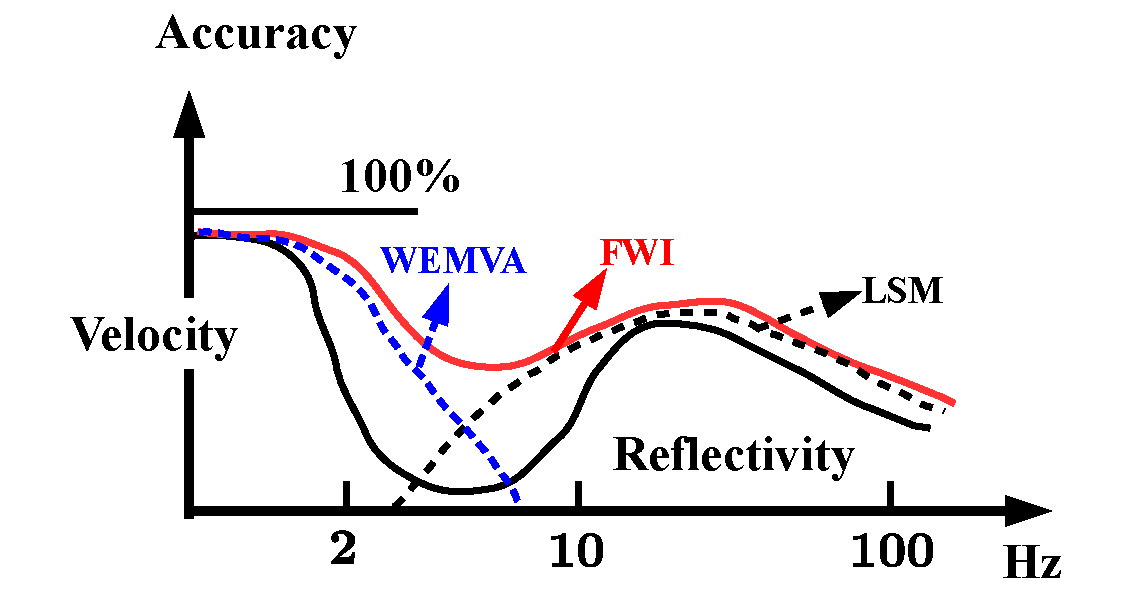
\includegraphics[width=1.00\textwidth]{Figure/chapter01/WavenumberGap1.pdf}}
   \caption{地震数据所能恢复的频带示意图,传统层析+成像的方式所恢复的速度频带中有着明显的中低频缺失,
   WEMVA和LSM方法能够分别拓展低波数与高波数部分的带宽,而FWI则尝试恢复更连续的波数谱。}
   \label{fig:GapInSeisVel}
\end{figure}

传统常规方法中大多基于射线类方法进行成像与速度估计,这在模型复杂区域很难处理多路径以及焦散等问题。而基于波动方程的方法则可以避免上述问题。
目前基于波动理论的主要反演方法主要有以下三类:

1、FWI,该方法通过匹配数据中携带的所有信息,包括走时、振幅、模式转换、多次波等等,来获得对地下模型的全波数谱的
恢复。
相比走时反演和MVA,它可以获取更高分辨率的地下模型。
因此自从Lailly(1983)\cite{lailly1983seismic}和Taratola(1984)\cite{tarantola1984}建立了FWI理论框架之后,随着宽频带,宽方位数据采集的成熟,FWI
被认为是填补速度模型中尺度波数成分空白的最强有力的工具。
但是FWI也受到众多的制约,如强烈的非线性程度(cycle-skipping),数据不完备导致的有限观测孔径,地下实际介质的非弹性以及各向异性,计算代价十分昂贵等等,因此
FWI虽经过数十年发展所面临的挑战依然十分艰巨;

2、波动方程偏移速度分析(WEMVA),该类方法旨在更新模型中的长波长背景速度,也即模型的低波数成分。
目前主流的做法通常利用数据中的反射波信息,通过获取反射波波路径信息来获得模型中深部的速度更新。
而根据其目标函数的残差类型又可以分为数据域反演(如Xu et al., 2012\cite{xu:2012};Wu and Alkhalifah,
2015\cite[]{Wu2015b}; Zhou et al, 
2015\cite[]{zhou:2015}; Chi et al, 2015\cite{chi2015})和扩展成像域反演(如Sava和Fomel, 2006\cite{Sava2006}; Almomin和Biondi, 2012\cite{Almomin2012})。
此类方法与基于射线理论的成像域层析与数据域(非线性)层析方法一脉相承,但是避免了传统层析流程中繁琐的人工拾取工作,不过其同样也会受困于cycle-skipping等问题;

3、最小二乘逆时偏移(LSRTM),该方法可以看作是线性化的FWI,在初始模型足够好的时候通过匹配模拟数据与观测数据的振幅来获得地下反射系数模型。常规偏移成像
采用伴随算子来近似正传算子的伪逆,从而近似地获得反射率的成像结果。但是伴随算子通常近似效果很差,最小平方偏移(LSM)通过迭代方式来获取正传算子的伪逆从而获得
更好的成像效果((Nemeth et al., 1999\cite{Nemeth1999},Kühl and Sacchi\cite{KuehlEtAl2003}, 2003,Dai,
2012\cite{DaiEtAl2012})。该过程可以看作是对目标函数对模型的二阶导数(也即Hessian)近似求逆的过程。

结合以上背景,如何恢复弹性介质中的速度模型将对勘探地球物理的发展至关重要。将弹性假设引入到以上反演问题中将会大大增加反问题的非线性程度。同时,多参数反演
也会带来参数间的耦合效应,这会进一步增加反演难度。由于计算机能力提升、多分量观测数据的增多以及解决声波FWI无法回避的问题的需要,考虑弹性甚至各向异
性的全波形反演逐渐成为研究热点。弹性波多分量数据中同时含有P波和S波,这两种不同波模式对地下介质有着不同的刻画作用。
近年来弹性波波模式分离技术能够提供准确的P或S波数据子集,这对反演中采取更多的多尺度策略带来可能性。董良国等(2015)\cite{董良国2015}
也指出在FWI过程中,不同的反演阶段采用不同的数据子集可以降低反演的非线性程度。而在弹性波反演中,更加需要根据不同参数
采用不同的数据子集或者不同的反演阶段
采用不同的数据子集,来降低多参数反演的非线性程度,同时也回避参数间的耦合效应。在本文中,
%通过模式解耦获取P或S波数据并根据
%需要加入到不同的反演阶段中,
%这种策略将贯穿始终,
模式解耦将在EFWI,弹性波波动放程反射走时反演(EWERTI)以及E-LSRTM中提供的分离的P或S波数据,来帮助获得更好的反演结果。
\section{研究现状}
\subsection{弹性波全波形反演研究现状}
Claerbout(1971\cite{Claerbout1971})采用爆炸发射面的概念解释了成像条件可以通过多次叠加来对地下构造进行刻画。Lailly(1983\cite{lailly1983seismic})
和Tarantola(1984\cite{tarantola1984})最早引入了表示观测数据与模拟数据间波形残差的$L_2$目标函数,将偏移成像的原理重新转化为寻优的
最优化问题,也即FWI。而该最优化问题的梯度方向可以采用共轭状态法通过入射波场与反传波场之间的互相关来快速获得。FWI试图将速度宏观模型的恢复(速度
建模)与偏移成像两个任务统一在一个流程中,这样就可以在地下每个网格点获得具有连续波数谱的高分辨率结果。但是早期只利用反射数据的FWI很少有令人满意的
结果,因为短偏移距观测的地震数据对中尺度波长的模型信息非常不敏感(Virieux and Operto, 2009\cite{virieux2009overview}),这就需要在初始模型非常准确
的时候FWI才能获得收敛。
从上世纪80年代末期,随着FWI在长偏移距以及井间透射波的应用成功,人们才发现FWI的潜力(Mora, 1987\cite{mora:1987}, 1988\cite{mora1988elastic}; Pratt
and Worthington, 1990\cite{PRATTEtAl1990}, Pratt et al., 1996\cite{pratt1996two})。
近年来在长偏移距、宽方位和宽频带采集的数据逐渐增多后,基于声波近似的FWI也在越来越多的实际数据中获得成功应用,例如Ravaut
et al., 2004\cite{RavautEtAl2004},Operto et al., 2006\cite{Operto2006},Shin et al.,
2009\cite{ShinEtAl2009}。然而即使对于含有长偏移距的数据而言,由于波传播路径的增加,非线性程度变得更加剧烈,因而从FWI中获得稳健的反演结
果仍然受到很大挑战(Sirgue, 2006\cite{sirgue2006importance},Virieux and Operto,
2009\cite{virieux2009overview})。

而从前文背景分析可以知道,最早始于Tarantola(1986)\cite{tarantola:1986}和Mora(1987)\cite{mora:1987}的弹性波全波形反演能够从多分量数据中反演地下介质的弹性参数,如P/S-波速度和密度。
尽管其仍然需要很大计算代价,EFWI还是在很多实际数据中获得了应用
Crase et al., 1992\cite{crase1992nonlinear}; Djikpesse and Tarantola,
1999\cite{djikpesse.tarantola:1999}; Sears et al., 2008\cite{sears2008}; Sear et al.,
2010\cite{sears:2010}; Prieux et al., 2013a\cite{prieux:2013a}, 2013b\cite{prieux:2013b}; Vigh et al.,
2014\cite{vigh:2014}。
EFWI的实现方式可以在时间域(Shipp et al., 2002\cite{shipp:2002}),
可以在频率域(Brossier et al., 2009\cite{brossier2009}),也可以采用混合的方式在时间域进行正演模拟而在频率域求解
(Nihei and Li, 2007\cite{nihei.li:2007}; Sirgue et al.,
2008\cite{sirgue:2008})。然而,EFWI中多个参数参与反演会增加反问题的非线性程度,同时也会受到由于不同物理参数之间的串扰带来的反演
中参数耦合的影响(Forgues and Lambare, 1997\cite{forgues.lambare:1997})。在海洋环境中,尤其是在软海底环境中,由于P-to-
S的转换模式非常弱,基于拖缆或者海底多分量数据的EFWI的非线性程度会变得更严重\cite{sears2008}。

从声波介质到弹性介质,波形反演方法将受到诸多挑战,解决EFWI中的问题,不仅要应对原有声波框架下的困难,同时也要解决多参数反演带来新问题。总的来说,
EFWI将主要面临以下两个方面的挑战:

1、反演的非线性,也即Cycle-skipping。FWI是基于Born近似的理论框架导出的。在Born散射下,Miller et
al(1987)\cite{MillerEtAl1987}基于ray+Born理论,
导出模型中散射点局部的波数矢量可以表达为:
\begin{equation}
    \mathbf{k}=\mathbf{k_s}+\mathbf{k_r}=\frac{\omega}{v}cos\frac{\theta}{2}\mathbf{n},
    \label{eq:Modelwnb}
\end{equation}
其中$\mathbf{k}$为照明矢量,$\mathbf{k_s}$和$\mathbf{k_r}$分别是震源端和检波点端的波场波数矢量,$v$为局部速度,$\theta$为散射角,
$\omega$为角频率,$\mathbf{n}$为$\mathbf{k}$方向的单位向量。由上式可以看出,低频和大孔径($\theta$)数据对于中低波数成分的恢复至关重要。
\begin{figure}[!htb] 
   \centering 
   \subfloat{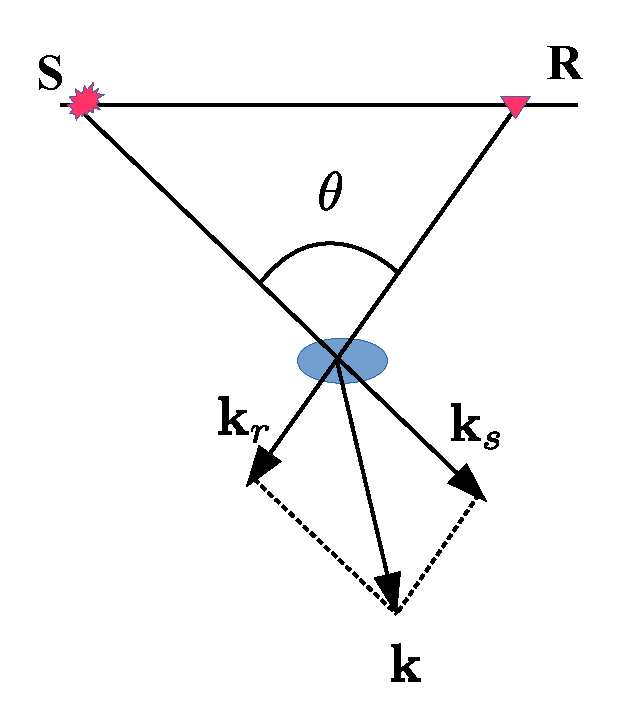
\includegraphics[width=0.40\textwidth]{Figure/chapter01/Wavenumbervector.pdf}}
   \caption{地下散射点处入射波矢量,散射波矢量以及散射角之间关系示意图。}
   \label{fig:WavenumberVector}
\end{figure}
\begin{figure}[!htb] 
   \centering 
   \subfloat{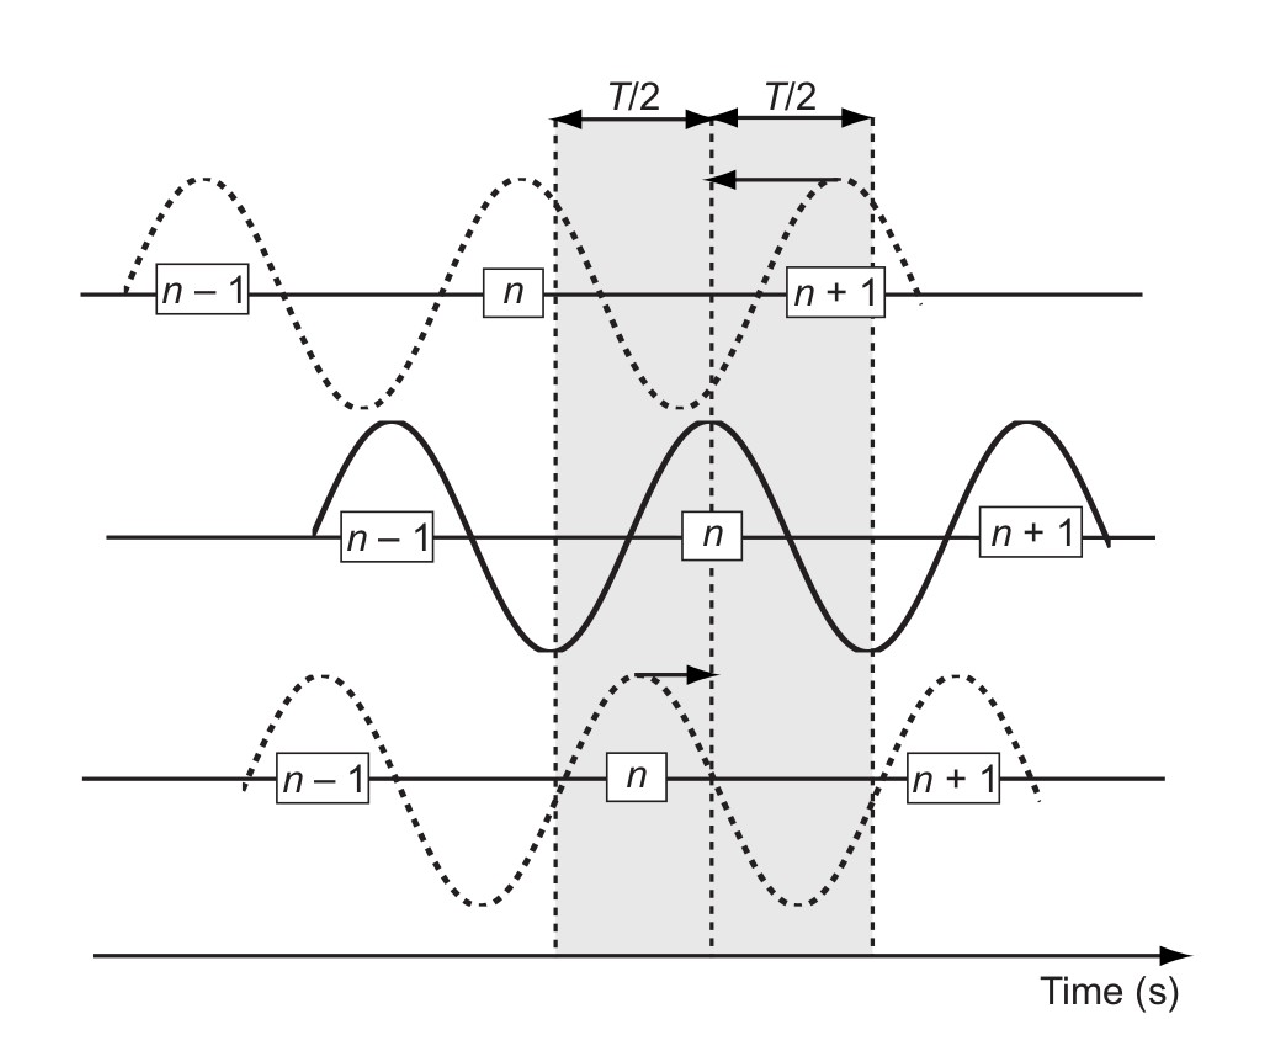
\includegraphics[width=0.60\textwidth]{Figure/chapter01/Cycle-skipping.pdf}}
   \caption{FWI波形匹配中的cycle-skipping现象。当波形相差$T/2$周期以上的时候,数据将会与在另一个周期中进行匹配,此时获得的数据残差会导致反演
   陷入局部极值。}
   \label{fig:Cycleskipping}
\end{figure}
因此FWI的成功与否非常依赖于长偏移距记录和数据中有效的低频分量。如图\ref{fig:Cycleskipping}
所示,如果初始模型不够好导致波形匹配时相差$\frac{1}{2}T$以上,那么就会使得反演陷入局部极值,这也就是所谓的“周波跳跃”问题。
在声波FWI中,发展了许多策略来解决非线性问题,如从低频到高频(Sirgue and
Pratt, 2004\cite{sirgue.pratt:2004}; 刘国峰等, 2012\cite{刘国峰2012};
刘璐等,2013\cite{刘璐2013}; 曹书红和陈景波, 2014\cite{曹书红2014}; 
张文生等, 2015\cite{张文生2015}),选取不同的时窗与偏移距逐步加入反演中(Shipp and
Singh, 2002\cite{shipp:2002}; Wang and Rao, 2009\cite{WangEtAl2009}; Sears,2008\cite{sears2008}),
修正目标函数使其凸性更好(Luo and Schuster, 1991\cite{luo1991};Tromp et al.,
2005\cite{tromp2005seismic};Chi
et al., 2014\cite{ChiEtAl2014}; Wu et al., 2014\cite{Wu2014b}; Shin and Cha,
2008\cite{shin.cha:2008}; Luo et al., 2016\cite{Luo2016})等等。这些策略可以用
在EFWI中,但是由于更多参数引入以及更复杂的弹性波波场,使得在使用这些策略的时候需要根据情况来择优选取。

而在EFWI中,不但会出现同样的强烈非线性,而且将面临更复杂的情况。
在构建初始模型的时候我们要同时获得足够好的$V_p$与$V_s$模型,这样才能对各种模式的转换波形进行
匹配。而$V_s$模型相比$V_p$初始模型更难获得。目前许多EFWI研究中都假设了$V_s$与$V_p$之间有着固定的Poisson比值的关系,因此可以通过简单的系数相乘
来构建初始模型。但是当地下介质Poisson比变化较大时很难获得较好的$V_s$初始模型,这就又增加了EFWI的困难。为了降低弹性波FWI非线性程度,许多学者通过
包络目标函数(黄超等,2015\cite{黄超2015},王官超和杜启振,2016\cite{王官超2016}),或者通过研究目标函数性态来指导多尺度策略的设计
(Brossier et al., 2010\cite{BrossierEtAl2010};王毓玮等,2016\cite{王毓玮2016})。
Tarantola(1986)\cite{tarantola:1986}指出EFWI应分主次顺序依次构建具有不同影响的参数。
或者采用多尺度策略多级的选取不同数据分量来进行反演(Sears, 2008\cite{sears2008}; Operto et al., 2013
\cite{operto2013guided})。然而实际中,诸多因素会制约这些策略的应用,例如低频缺失,初始模型不够好,子波估计,噪音等等。因而降低EFWI的非线性
程度使得反演更加稳健可靠依然需要诸多努力。

2、多参数反演中的参数耦合效应。如果物理模型中引入多个参数,那么不同的参数扰动可能会引起相似的数据扰动。虽然其产生的数据扰动可能不完全一致,
但是不同参数的“偏导数波场\cite{pratt1998gauss}”会在特定角度范围内的重叠,这就导致无法简单地区分开数据扰动来自哪一种
参数扰动,从而引起参数间的耦合效应。这样的话,即使在初始模型足够好的时候也很难从数据扰动中恢复其相应的参数扰动。

为了解决EFWI中的参数耦合问题,
许多学者通过调查散射模式或者Hessian算子来选取不同的参数化方式(Wu and Aki, 1985\cite{wu.aki:1985};Tarantola, 1986\cite{tarantola:1986};
Plessix and Cao, 2011\cite{plessix.cao:2011},Gholami et al, 2013\cite{gholami2013})。
当然最有效的就是考虑多参数Hessian算子的方法,用Hessian的信息来压制参数耦合的影响(Fichtner et al., 2001\cite{fichtner2011hessian};Operto et al.,
2013\cite{operto2013guided},Pan et al., 2015\cite{pan2015estimation};Yang et al.,
2016\cite{Yang2016})。然而由于Hessian计算所需代价太过于昂贵,即使在声波FWI也很难在大规模问题中获得应用。在EFWI中想要获得压制参数耦合的效果,就
需要在反演中包含对Hessian的非对角区块的近似。近期,在Hessian非对角区块的近似与利用方面,许多学者都将其应用到了EFWI中,例如Wang
et al.(2016)\cite{WangEtAl2016}采用块对角Hessian压制参数耦合,Pan et
al(2017)\cite{PanEtAl2017}采用Hessian-free的方式采用l-BFGS的优化策略进行多参数反演,Wang and Cheng
(2017)\cite{WangEtAl2017}指出模式解耦可以部分的利用Hessian非对角块来压制P波对$V_s$反演的干扰。而于此同时EFWI中,由于密度参数对数据不敏感,因此密度
的反演依然很难获得令人满意的结果。
\subsection{弹性反射波波形反演研究现状}
尽管常规FWI在长偏移距,宽方位数据中有着令人满意的效果,但是在这种观测系统下,FWI主要利用了长偏移距透射波以及临界反射波所携带的信息来更新速度模型的
中长尺度波长的分量。由于FWI的成功非常依赖这种透射信息,就会使得FWI往往缺乏足够的大偏移距信息来更新模型中深部结构的中低波数成分。
这就导致在深部的区域,FWI往往只能更新来自反射数据的高波数成分(也即是最小平方偏移的过程)而很难更新中低波数成分。从式\ref{eq:Modelwnb}
中也可以看出,在相同频率和速度下,深部的反演需要更大的角度覆盖才能确保足够的低波数照明,这也意味着要更大的偏移距。然而即使对
于目前宽方位长偏移距的采集技术也很难保证这样的覆盖,况且更长的偏移距也意味着更强的非线性\cite{sirgue2006importance,virieux2009overview}。

利用反射波信息可以更好的照明深部,通常可以在成像域或者数据域实现深部的速度更新。在成像域,该类方法通常被称为偏移速度分析(MVA),其主要利用拉平
共成像点道集作为收敛准则。
在实际生产中,通过射线走时层析来利用反射波信息更新中深部的背景速度已经是非常成熟的技术(Woodward,
1992\cite{Woodward1992}; Meng et al., 2004\cite{MengEtAl2004};Woodward et al.,2008\cite{
Woodward2008}; Jones, 2010\cite{Jones2010})。
其通过将道集上的剩余时差(或深度差)反投影到射线路径上来获得速度更新。不过射线层析经常需要进行许多人工干预,尤其是在每轮迭代中进行
成像剖面与成像道集的拾取。而且在构造复杂区域,射线高频渐近近似失效,使得走时层析很难获得成功。
基于波动理论的成像域偏移速度分析(WEMVA)可以很好的回避上述问题,但是其通常
需要引入扩展成像条件,通过最小化扩展道集上非零偏移距的能量来实现更新,如Sava and
Fomel(2006)\cite{SavaEtAl2006}; Yang and Sava(2011)\cite{YangEtAl2011}; Almomin and
Biondi(2012)\cite{Almomin2012}; Sun and Symes(2012)\cite{SunEtAl2012}。尽管WEMVA在
二维应用中取得了不错的效果,但其主要缺陷就是计算代价太过昂贵,尤其实在三维问题中,一方面偏移成像需要大量计算,
另一方面扩展成像条件的施加同样耗费极大。
针对反射走时,Luo et
al(2016)\cite{Luo2016}用时间轴方向的扩展成像与Rytov近似结合,导出了全走时反演(FTI)获得了不错的反演效果,但其实质上也是一种成像域的反演方法。

在数据域同样可以实现反射波对模型的深部更新。
许多学者(Chavent et al, 1994\cite{ChaventEtAl1994}; Plessix et al.,1998\cite{PlessixEtAl1998}; Clment et al.
,2001\cite{ClementEtAl2001})将速度模型分成高波数(反射率)与低波数成分(背景模型),提出了偏移成像走时层析(MBTT)。
从Woodward et
al.(2008)\cite{Woodward2008}和Alder(2008)\cite{Adler2008}提出的基于射线理论的非线性层析方法出发,Wang
et al\cite{WangEtAl2014}和Yang et al\cite{YangEtAl2016}采用一次偏移后拾取+图偏移的方式建立叠前数据的不变量(如走时,相位,出射慢度等),从而实现对
叠前数据的多次非线性拟合,进而减少人工拾取工作量达到加快速度的效果。基于波动理论的数据域速度建模近年来受到了广泛的关注。
受MBTT方法的启发,Xu et al (2012)\cite{xu:2012}提出了反射波波形反演方法(RWI)。RWI先采用RTM或LSRTM的方式获取反射率,
然后用Born模拟来预测反射率所产生的反射波,而反射波与背景波场的互相关就可以得到反射波波路径信息。
RWI思想的关键就是将数据域中通过不同目标函数获得的数据残差反投影到反射波波路径上,从而更新中低波数成分的模型分量。
RWI的思想产生后,许多学者针对不同的目标函数选取方法做了很多研究。许多RWI研究都采用波形拟拟合的$L_2$范数,如Xu
et al (2012)\cite{xu:2012}, Wang et al(2013)\cite{Wang2013}, Wu and
Alkhalifah(2015)\cite{Wu2015b},
Zhou et al(2015)\cite{zhou:2015}。然而尽管RWI的目的在于更新背景速度,波形拟合的$L_2$范数在背景速度与真实值相差较远的时候,反射率所预测的反射波与
观测数据中的反射波波形相差半个周期以上的时候,仍然会产生周波跳跃。Wang et
al(2013)\cite{Wang2013}指出采用低频数据可以一定程度上避免跳周现象。为了避免振幅相关的目标函数带来的非线性,与背景速度更具有线性关系的
走时类的目标函数也获得了关注。Ma and
Hale(2013)\cite{ma2013}采用动态图像识别(DIW)来获得模拟与观测反射数据之间的时移,从而导出了波动方程反射走时反演(WERTI)。Chi
et al (2015)\cite{chi2015}和Wang et al
(2015)\cite{Wang2015}采用互相关类的方法来获取时移(或空移)。而近期,Irabor and
Warner(2016)\cite{Irabor2016}和Wang et al(2016)\cite{WangEtAl2016}通过上下形波分离来获取常规FWI中的背景更新分量,但其实质上也利用了反射波波路径的信息。

以上RWI的研究现状都是基于声波方程得出的。在弹性波反射波形反演中,目前只有Guo and
Alkhalifah(2016)\cite{Guo2016}将Wu and
Alkhalifah(2015)\cite{Wu2015b}的思路扩展到了弹性介质中,而其他方法在弹性介质中的应用则
基本没有研究触及到。在弹性介质中,除了声波介质中面临的问题,ERWI还需要处理更多的复杂情况,如多参数,模式转换,更复杂的反射记录以及
$V_s$结构中成像与反演的困难等等诸多挑战。为了解决这些问题,利用波模式解耦来分别获取P与S反射波然后应用到声波对应的方法中将是非常直观的思路,但是
这都需要考虑到弹性波的特殊情况,处理好每种方法相应的问题才能获得可行的ERWI方案。
%许多研究通过选取不同的目标函数来选取方法对应不同名称的反演方法,但核心思想都是一致的

\subsection{弹性波最小平方逆时偏移研究现状}

目前有许多成像方法,如Kirchhoff偏移,高斯束偏移,RTM等等可以用来恢复地下界面结构。但是随着技术进步,界面构造信息已经不能满足勘探的需要,我们想要
获得更准确的高波数成分。
常规的FWI算法可以高分辨率地恢复模型的高波数成分,但是会受到许多因素干扰,
如cycle-skipping问题,信噪比低,地震子波未知,正演算子不准确等等。
而且常规FWI需要从低频到高频逐步恢复连续的波数谱,如果我们单纯想获得模型高波数成分,
用FWI方法就太过复杂。除FWI之外,我们通常也会通过最小平方偏移(LSM)来实现高波数成分的重构。
早期,Beylkin
et al(1985)\cite{BeylkinEtAl1985}以及
Bleistein(1987)\cite{Bleistein1987}等学者通过广义Radon变换来导出Kirchhoff成像中的振幅校正因子,也即真振幅成像技术。该方法通过射线理论计算Green函数,正问题采用Born近似
计算,进而快速的迭代求解反问题。
针对Kirchhoff偏移,Schuster(1993)\cite{Schuster1993}提出了应用于井间数据的LSM算法,而Nemeth et al.\cite{Nemeth1999}将该方法应用到了地面数据中。
以波动方程为引擎的最小平方逆时偏移(LSRTM)近年来一直是研究的热点,
尽管其计算代价昂贵,但是LSRTM可以回避模型速度复杂时所产生的多路径问题。
LSRTM的过程通常被认为是线性的全波形反演,理论上施加Hessian矩阵的逆就可以获得最终的反演结果。但是Hessian的计算与求逆在实际问题中基本无法实现,
在空间域采用Hessian的近似来校正成像结果是一种快速获得LSRTM结果的方法(Chavent and Plessix, 
1999\cite{ChaventEtAl1999}; Shin et al., 2001\cite{shin2001improved}; Symes,
2008\cite{Symes2008}),然而这种方法在复杂区域并
不总是有效。另外一种方式是通过在数据域求解目标函数的最优化问题其假设在已经获得足够好的低波数模型成分之后恢复模型的高频扰动,也即获得“像”或
反射率,使得在最小平方意义下,用该反射率所预测的反射数据能与观测数据达到最佳匹配。这一过程与在单次迭代中通过计算二阶伴随状态方程来使用
Gauss-Newton法(Bae et al., 2012\cite{bae2012frequency};Metiver et al.,
2014\cite{Metivier2014})求解FWI是一致的。
因此,最小平方逆时偏移与全波形反演的理论框架是一致的,只是输入数据(反射波与全波场)和输出结果(高频扰动与模型参数)不一样。
因此目前LSRTM研究的主要方式通过最小化Born模拟的反射数据与观测数据之间的残差来改善成像质量、获得更高分辨率的结果(Dai and
Schuster(2013)\cite{Dai2013},Dong et al.(2012)\cite{Dong2012}, Luo and
Hale(2014)\cite{Luo2014})。

许多学者针对LSRTM中的不同问题做了大量的研究工作。Wong et al.
(2015)\cite{WongEtAl2015}将自由表面多次波加入到成像条件中,进而增加地下照明。Zhang et al.
(2015)\cite{ZhangEtAl2015}选取零延迟互相关目标函数来减弱子波估计不准以及振幅描述不准带来的非线性。刘玉金和李振春
(2015)\cite{刘玉金2015}基于成像域的速度反演方法(Symes,2008\cite{Symes2008a})
在扩展域进行LSRTM,这样即使在速度不准确的情况下仍然可以得到合理的成像结果。
近期,为了更准确地描述波传播过程,同时获得更多的参数成像,并解决多参数带来的耦合效应,原本基于声波方程的
LSRTM被推广到了变密度声波介质(Yang et al, 2016)\cite{Yang2016}),衰减介质(Dutta and
Schuster, 2014\cite{DuttaEtAl2014}; 李振春等,2014\cite{李振春2014}; Dai et al,.
2015\cite{Dai2015})以及弹性介质中(Duan et al., 2016\cite{Duan2016};Feng and Schuster,
2016\cite{Feng2016}; Xu et al., 2016\cite{Xu2016};Ren et al., 2016\cite{RenEtAl2016})。

相比声波成像,弹性波成像可以提供更多的地下信息,例如裂缝分布以及弹性性质。但是,弹性波偏移中存在的许多问题会很大程度上影响成像质量。因为通常很难将
记录中的 
波模式完全区分开,因此其中某些波模式的会因速度不对而被错误地成像。这些非物理的模式就会引起假象,也即“cross-talk”。
而通过ELSRTM则可以提高成像的分辨率,并且可以压制由于观测孔径限制,粗网格采样以及数据缺失引起的偏移假象。
弹性波成像需要处理矢量波的问题,也就需要选取合适的成像条件(Du et al, 2014\cite{DuEtAl2014};Gong et
al, 2016\cite{GongEtAl2016};Rocha et al,2016\cite{RochaEtAl2016a}),近期Wang et
al(2016)\cite{WangEtAl2016}提出了更具有物理含义的无极性反转
的矢量成像条件。

而从EFWI理论框架出发,许多学者,
如Duan et al.(2016)\cite{Duan2016},Feng et
al.(2016)\cite{Feng2016}
等都推导出了与EFWI梯度非常类似的成像条件。该成像条件也可以回避极性反转问题,同时也可以认为是更加接近于高频的参数扰动梯度。而基于
第二章中对EFWI算法的分析,模式解耦带来的优势将同样能在ELSRTM中得以应用。


\section{研究内容}
弹性参数的恢复与重构将是本文的重点。
目前主流的估计模型参数的方法包括FWI、RWI和LSRTM,
我们将以上三个方法扩展到弹性介质来研究与估计模型参数,其非别对应为EFWI构建高分辨率速度模型,E-WERTI构建中深部中低波数的背景速度,
E-LSRTM构建模型高波数成分。而整个论文中,弹性波模式解耦将贯穿始终,来为每种方法提供不同的数据子集以及降低参数耦合的便利。
因此本论文将分为以下四个部分来详细阐述:

第二章将通过模式解耦来对EFWI梯度进行预条件来降低反演过程中的参数耦合程度,并达到加速收敛的效果。
首先,通过弹性波Born近似,我们将分析P波速度与S波速度扰动的
辐射模式,并导出解耦的Frech{$\acute{e}$}t导数或Jacobian矩阵;然后,我们将调查解耦后的P波与S波数据对梯度的贡献并提出在梯度计算中的交叉项近似。
在此基础上,预条件的梯度可以通过伴随状态法\cite[]{plessix2006}快速有效地计算得到,也即正传波场与解耦后反传波场的零延迟互相关。
然后,为了获得更多物理机制上的认识,我们计算并分析基于解耦的Hessian和分辨率矩阵,同时也对比MD预条件后的梯度与GN梯度的异同。
此后,流体饱和沙岩模型以及Marmousi-II模型的数值实验验证基于解耦的EFWI的有效性。
最后,我们将给出关于密度反演的简单讨论与结论。

第三章将通过弹性波波动方程反射走时反演(E-WERTI)来重建速度模型中深部的中低波数分量。
文中采用走时作为目标函数进行反演,反射波的走时差将通过DIW来获取。
采用RWI的思路通过Born模拟来构建反射波关于背景速度的核函数,也即反射波波路径。
由此参照Ma and Hale\cite{ma2013}的方式,导出弹性波方程中对应的反射走时反演梯度与伴随震源。
在文中,我们首先通过目标函数的形态分析调查E-WERTI的稳健性与收敛性。然后分析反射核函数的形态观察不同反射波波模式对反射路径的影响。
为了克服P波与S波速度之间的耦合性,我们将分成两个阶段来分别恢复P波与S波速度:首先采用PP波反射走时来重构出P波速度的背景模型,
在获得足够的P波背景速度后,固定P波速度背景模型,采用分离出的PS波反射信息来重构S波速度背景模型。
在此过程中,采用地面P/S数据分离来获取P或S波多分量地震记录,采用空间波场分解来计算P或S波的梯度
最后算法将在Sigsbee2A模型上进行实验验证。

第四章将采用弹性波LSRTM来获取模型的高波数分量。首先,我们从反演框架出发,建立模拟与观测反射数据之间的最小二乘目标函数,
利用矩阵形式的弹性波方程通过Lagrangian乘子法获得伴随状态方程,并导出E-LSRTM的梯度。
之后根据第一章的推导,利用波模式解耦对导出的梯度进行预条件来降低参数耦合效应。
由于E-LSRTM基于Born近似假设,Born正演数据与反射数据之间将存在差异,文中对比采用不同偏移模型E-LSRTM时
Born数据与反射数据所得反演结果产生的差异。
LSRTM为线性FWI过程,反问题的复杂程度将大为降低,我们将对比不同的策略来解决参数耦合问题。
简单模型与Marmousi的数值实验将用来验证算法的有效性。

第五章中,将对本文的工作进行总结,讨论论文的创新与不足之处,并规划下一步的研究重点。
